\label{sec:background}
\subsection{CNN based methods in DSLAM}
As described before, there are two essential components on each agent: 1) Visual Odometry (VO) and 2) Place Recognition.

\subsubsection{Visual Odometry (VO)}



\subsubsection{Place Recognition}

The goal of place recognition is to calculate a given frame into a limited set of places. Each places can be encoded as a very short code which can be easy tranformed with low communication cost. Tranditional place recognition method usually translate the input frame as the aggregation of handcrafted feature point and local descriptors, like SIFT \cite{Lowe:2004e6e} or ORB \cite{Mur-Artal:2017281}, using vectorization techniques like bag-of-words (BoW) \cite{Galvez-Lopez:2012c94} or vector of locally aggregated descriptors(VLAD) \cite{Jegou:2010f45}.

Recent advances in the deep learning and the convolution neural network (CNN) enable powerful end-to-end mode for place recognition \cite{Noh:2017d0b,Arandjelovic:2017997}, and the NetVLAD method is one of the most accurate method based on CNN. The NetVLAD algorithm based on VGG-16 model \cite{Simonyan:20143be} consumes more than $80G$ operations for a single $300 \times 300$ input image (each operation means an addition or a multiplication). It is very challaging to deploy the NetVLAD on a tranditional embedded hardware platform.

\subsection{Hardware architecture of Zync SoC}
The Xilinx Zync Soc is a chip with ARM cores and FPGA fabric. The system is illustrated in \cref{fig:plps}. The ARM cores with an embedded Linux operation system are called Processing System (PS). The FPGA fabric is called Programmable Logic (PL). The peripherals like camera and communication unit (WiFi or others) are accessable with PS. The high-bandwidth on-chip AXI interface is used to communicate between PS and PL. PS and PL can also share the DDR to transfer large volume of data such as each frame of camera.
Deephi CNN accelerator \cite{Tech:2019360} is one of the state-of-the-art accelerators and is famous for high energy efficiency on various of CNN structure. We deploy the accelerator on the PL side of Zynq SoC.

\begin{figure}[thb]  
    \centering  
    {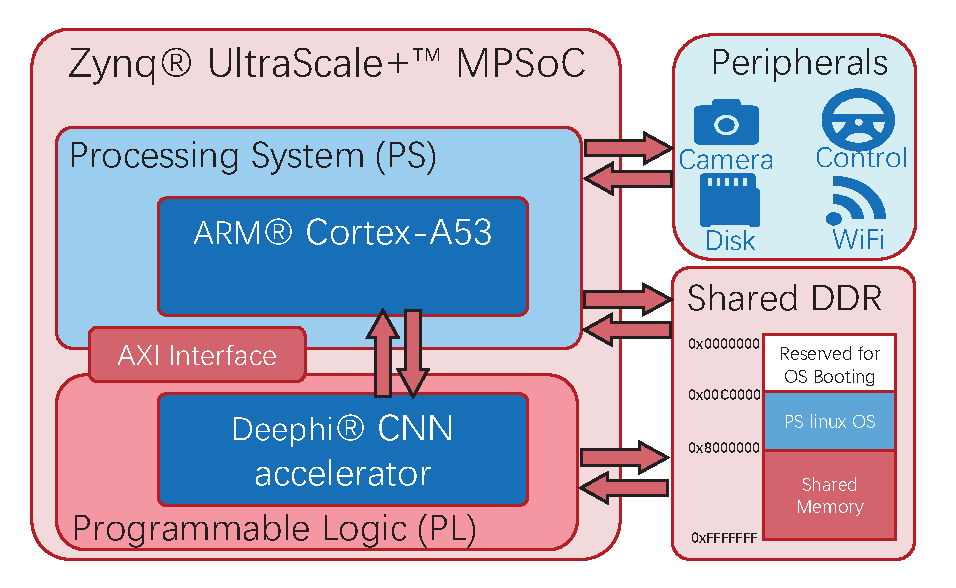
\includegraphics[width=0.95\linewidth]{fig/plps.eps}\label{fig:plps}} 
    \caption{Hardware architecture of Zynq SoC}
\end{figure}

Though FPGA can greatly improve the performance and energy efficiency of CNN inference, FPGA cannot efficiently calculate float-point number and requires fixed-point parameters and intermediate data in CNN.